\documentclass{beamer}

\usepackage{changepage}
\usepackage{hyperref}

\usepackage[skip=0.2\baselineskip]{parskip}

\usepackage{mathrsfs}
\usepackage{caption}
\usepackage{subcaption}
\usepackage{tikz}
\usepackage{makecell}
\usepackage{array,booktabs}

\usepackage{bm}

\newcolumntype{C}{>{$\displaystyle}c<{$}}

\setlength\fboxsep{0pt}
\setlength\fboxrule{0pt}


\usepackage{theme/beamerthemepamango-blank}
\usepackage{shortcuts_pm}


\setbeamertemplate{caption}{\raggedright\insertcaption\par}

\addbibresource{references.bib}

%%%%% INFORMATION

\title{\huge High-Dimensional Private ERM \\ by Greedy Coordinate Descent}
\author{
  Paul Mangold \\[1em]
 Supervised by \\ Aurélien~Bellet, Marc~Tommasi, and Joseph~Salmon
}
\institute{\textsc{LOL 2022}}

\date{October 3th, 2022}

%%%%% DOCUMENT

\begin{document}

%% TITLE PAGE

\begin{notitle}
  \begin{frame}
    \titlepage
  \end{frame}
  \addtocounter{framenumber}{-1}
\end{notitle}


% \hspace{-3.3em}
% \begin{frame}
%   \vspace{-7.7em}
%   \includegraphics[width=1.17\textwidth]{example_none.pdf}

%   \vspace{-18em}
%   \begin{align*}
%     \qquad \qquad ~ \min_{w\in\RR^p} f(w)
%     & = \frac 1n \sum_{i=1}^n \ell(w; d_i)
%   \end{align*}
% \end{frame}

% \hspace{-3.3em}
% \begin{frame}
%   \vspace{-1.8em}
%   \includegraphics[width=1.17\textwidth]{example_1_nopriv.pdf}
%   \addtocounter{framenumber}{-1}
% \end{frame}

% \hspace{-3.3em}
% \begin{frame}
%   \vspace{-1.8em}
%   \includegraphics[width=1.17\textwidth]{example_2_nopriv.pdf}
%   \addtocounter{framenumber}{-1}
% \end{frame}

% \hspace{-3.3em}
% \begin{frame}
%   \vspace{-1.8em}
%   \includegraphics[width=1.17\textwidth]{example_3_nopriv.pdf}
%   \addtocounter{framenumber}{-1}
% \end{frame}

\begin{frame}
  \vspace{2em}

  {\Huge
    \textit{Differentially Private} ERM:
  }

  \vspace{-1em}

  \begin{align*}
    & \argmin_{w \in \RR^p}  f(w) = \frac 1n \sum_{i=1}^n \ell(w; d_i) \\
    & \qquad \text{\emph{such that $w$ is $(\epsilon, \delta)$-DP}}
  \end{align*}
  {
    \begin{center}
      (with $\ell$ convex, Lipschitz and smooth)
    \end{center}
  }
%  \smalllongcite{chaudhuri2011Differentially}
\end{frame}

% \begin{frame}
%   \vspace{2em}

%   $\emphcolb{\cA} : D \mapsto w$ is
%   $(\emphcol{\epsilon}, \emphcol{\delta})$-\textit{Differentially
%     Private}
%   \begin{align*}
%     \prob{\emphcolb{\cA}(D) \in \cS} \le e^{\emphcol{\epsilon}} \prob{\emphcolb{\cA}(D') \in \cS} + \emphcol{\delta}
%   \end{align*}

%   \vspace{1em}

%   \begin{flushright}
%     ($D$ and $D'$ differ on one element)
%   \end{flushright}

%   \smalllongcite{dwork2006Differential}
% \end{frame}



% \begin{frame}
%   \vspace{-0.3em}
%   \includegraphics[width=1.17\textwidth]{example_1.pdf}
%   \addtocounter{framenumber}{-1}
% \end{frame}

% \hspace{-3.3em}
% \begin{frame}
%   \vspace{-0.3em}
%   \includegraphics[width=1.17\textwidth]{example_3.pdf}
%   \addtocounter{framenumber}{-1}
% \end{frame}


% \begin{frame}
%   \vspace{3em}

%   {\Huge Private Gradient Descent}
%   \begin{align*}
%     w^{t+1} = w^t - \eta
%     \left(  \emphcol{\nabla f(w^t)} + \emphcolb{\cN(\sigma^2\bbI)} \right)
%   \end{align*}

%   With $\displaystyle\emphcolb{\sigma^2} \propto \frac{\emphcol{Tp}}{n^2\epsilon^2}$

%   \vspace{0em}
%   \longcite{bassily2014Differentially}
% \end{frame}

% \begin{frame}
%   \vspace{0.5em}

%   {\Huge Private Coordinate Descent}
%   \begin{align*}
%     & \text{Choose }j \sim_u \{1, \dots, p\} \\
%     & \text{Update } \\
%     & \quad w^{t+1}_{j} =
%       w^t_{j} - \eta_{j}
%     \left( \emphcol{\nabla_{j} f(w^t)}
%     + \emphcolb{\cN(\sigma_{j}^2)} \right)
%   \end{align*}
%   With $\displaystyle\emphcolb{\sigma_j^2} \propto \frac{\emphcol{T}}{n^2\epsilon^2}$

%   \vspace{-0.7em}
%   \longcite{mangold2021ifferentially}
% \end{frame}


% \hspace{-3.3em}
% \begin{frame}
%   \vspace{-0.3em}
%   \includegraphics[width=1.17\textwidth]{example_1.pdf}
% \end{frame}


% \hspace{-3.3em}
% \begin{frame}
%   \vspace{-0.3em}
%   \includegraphics[width=1.17\textwidth]{example_2.pdf}

%   \addtocounter{framenumber}{-1}
% \end{frame}



% \begin{frame}
%   \Huge
%   Utility: $\expec{}{f(w) - f^*} = \text{ ?}$

%   \vspace{0.5em}

%   {
%     \begin{center}
%       \huge   (when $f$ and $\nabla f$ are Lipschitz)
%     \end{center}
%   }

%   \pause
%   \vspace{1em}

%   \begin{itemize}
%   \item Convex: $\widetilde O\left( \frac{\emphcol{\sqrt{p}}}{n\epsilon} \right)$
%   \item Strongly-Convex:  $\widetilde O\left( \frac{\emphcol{p}}{n^2\epsilon^2} \right)$
%   \end{itemize}
% \end{frame}


% \begin{frame}
%   ~
%   \begin{center}
%     \Huge
%     Can we choose updates ``wisely''?
%   \end{center}
% \end{frame}

\begin{frame}
  \vspace{2em}

  {\Huge Private \emph{Greedy} CD}
  \begin{align*}
    & \text{Choose} \\
    & \quad j = \argmax_{j'\in[p]} \abs{\emphcol{\nabla_{j'} f(w^t)} + \emphcolb{\Lap(\lambda_{j'}')}} \\
    & \text{Update} \\
    & \quad w^{t+1}_{j} =
      w^t_{j} - \eta_{j}
    \left( \emphcol{\nabla_{j} f(w^t)}
    + \emphcolb{\Lap(\lambda_{j})} \right)
  \end{align*}
\end{frame}
% \begin{frame}
%   \vspace{1em}

%   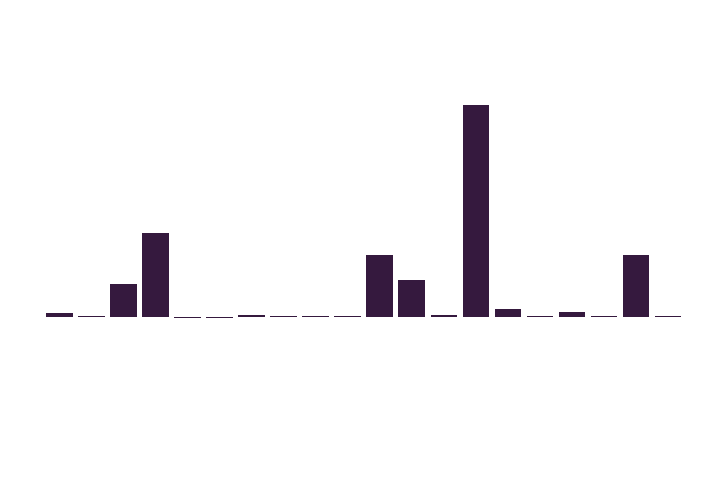
\includegraphics[width=\textwidth]{grad_example_1.pdf}

%   \vspace{-2em}

%   \begin{center}
%     \phantom{\Huge \emph{noise variance} $\propto Tp/n^2\epsilon^2$}
%   \end{center}
% \end{frame}

% \begin{frame}
%   \vspace{1em}

%   \includegraphics[width=\textwidth]{grad_example_2.pdf}

%   \vspace{-1.5em}

%   \begin{center}
%     \Huge \emph{noise variance} $\propto Tp/n^2\epsilon^2$
%   \end{center}
%   \addtocounter{framenumber}{-1}
% \end{frame}

% \begin{frame}
%   \vspace{1em}

%   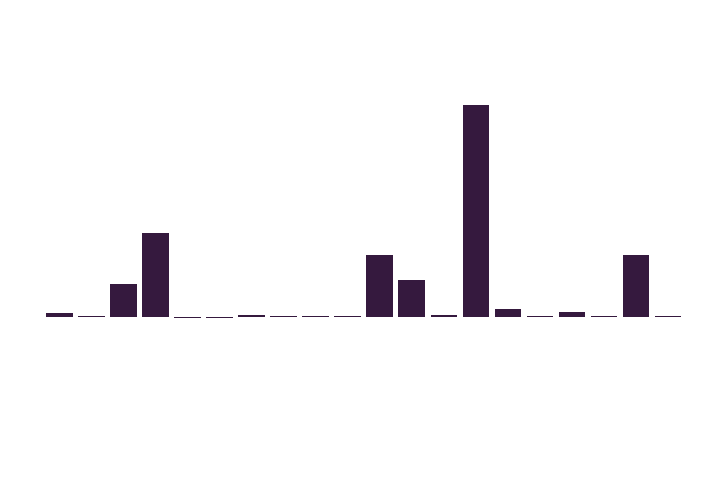
\includegraphics[width=\textwidth]{grad_example_1.pdf}

%   \vspace{-2em}

%   \begin{center}
%     {\Huge Release only the maximum?}
%   \end{center}
% \end{frame}


% \begin{frame}
%   \vspace{1em}

%   \includegraphics[width=\textwidth]{grad_example_noisy_1.pdf}

%   \vspace{-1.5em}

%   \begin{center}
%     \Huge \emph{noise variance} $\propto T/n^2\epsilon^2$
%   \end{center}
%   \addtocounter{framenumber}{-1}
% \end{frame}

% \begin{frame}
%   \vspace{1em}

%   \includegraphics[width=\textwidth]{grad_example_3.pdf}

%   \vspace{-1.5em}

%   \begin{center}
%     \Huge \emph{noise variance} $\propto T/n^2\epsilon^2$
%   \end{center}
%   \addtocounter{framenumber}{-1}
% \end{frame}


% \hspace{-3.3em}
% \begin{frame}
%   \vspace{-0.3em}
%   \includegraphics[width=1.17\textwidth]{example_3.pdf}
% \end{frame}





% \begin{frame}
%   \vspace{1em}
%   \Huge
%   Utility: $\expec{}{f(w) - f^*} = \text{ ?}$

%   \vspace{0.5em}
%   {
%     \begin{center}
%       \huge   (when $f$ and $\nabla f$ are Lipschitz)
%     \end{center}
%   }

%   \pause

%   \vspace{1em}
%   \begin{itemize}
%   \item Convex: $\widetilde O\left( \frac{\emphcol{\log{p}}}{n\epsilon} \right)$
%   \item Strongly-Convex:  $\widetilde O\left( \frac{\emphcol{\log{p}}}{n^2\epsilon^2} \right)$
%   \end{itemize}

%   \vspace{.5em}
%   \begin{center}
%     \huge
%     Under favorable structure
%   \end{center}

% \end{frame}

% \begin{frame}
%   \vspace{-0em}
%   {
%     \begin{center}
%       \Huge Fast Initial Progress
%     \end{center}
%   }
%   \begin{center}
%     for $\mu_2$-strongly-convex $f$, $L$-Lipschitz $\nabla f$, \\[-0.5em] \emph{worst case}
%   \end{center}
%   \vspace{-0.5em}

%   \begin{align*}
%     %    \label{gcd:fast-initial-convergence:eq}
%     \!\!\!\!f(w^T) - f^*
%      & \!\le \prod_{t=1}^T \Big(1 - \frac{\mu_{2}}{4L\emphcol{p}}\Big) (f(w^0) - f^*) \\
%     & \quad + O\Big(\frac{T}{\mu_{2} n^2 \epsilon^2}\Big)
%   \end{align*}

%   \vspace{0.5em}
% \end{frame}

% \begin{frame}
%   \vspace{-0em}
%   {
%     \begin{center}
%       \Huge Fast Initial Progress
%     \end{center}
%   }
%   \begin{center}
%     for $\mu_2$-strongly-convex $f$, $L$-Lipschitz $\nabla f$, \\[-0.5em] \emph{$\tau$-sparse solution}
%   \end{center}
%   \vspace{-0.5em}

%   \begin{align*}
%     %    \label{gcd:fast-initial-convergence:eq}
%     \!\!\!\!f(w^T) - f^*
%      & \!\le \prod_{t=1}^T \Big(1 - \frac{\mu_{2}}{4L\emphcol{(t + \tau)}}\Big) (f(w^0) - f^*) \\
%     & \quad + O\Big(\frac{T\emphcol{(T+\tau)}}{\mu_{2} n^2 \epsilon^2}\Big)
%   \end{align*}

%   \vspace{0.5em}

%   \begin{center}
%     \Huge Fast when $T+\tau \ll p$
%   \end{center}
% \end{frame}


% \begin{frame}
%   \begin{center}
%     Logistic Regression ($n=1000,p=100$)

%     $w^* \sim \text{lognormal}(\sigma=1)^p$
%     \only<1>{
%       \includegraphics[width=0.8\textwidth]{lognormal_solution.pdf}
%     }
%     \only<2>{
%       \includegraphics[width=0.8\textwidth]{plots_final/lognormal_opt_1_norm.pdf}
%     }
%   \end{center}
% \end{frame}

% \begin{frame}
%   \begin{center}
%     Logistic Regression ($n=1000,p=100$)

%     $w^* \sim \text{lognormal}(\sigma=2)^p$

%     \includegraphics[width=0.8\textwidth]{plots_final/lognormal_opt_2_norm.pdf}
%   \end{center}
% \end{frame}

\hspace{-3.3em}
\begin{frame}
  \vspace{-0.3em}
  \includegraphics[width=1.17\textwidth]{example_3.pdf}
\end{frame}


\begin{frame}
  \begin{center}
    Logistic Regression ($n=2600, p=500$)

    \vspace{-0.5em}

    \texttt{madelon} dataset

    \vspace{0.5em}

    \includegraphics[width=0.8\textwidth]{plots_final/madelon_l2_norm.pdf}
  \end{center}
\end{frame}

\begin{frame}
  {
    \begin{center}
      \Huge Open Questions!
    \end{center}
  }

  \vspace{-1em}

  \Huge
  \begin{itemize}
  \item Proximal Greedy CD?
  \item Sparse solutions?
  \end{itemize}

\end{frame}

% \begin{frame}
%   \begin{center}
%     \vspace{4em}

%     \Huge
%     Thank you!

%     % \vspace{2em}

%     % \huge
%     % Come see our poster! :)

%     % \vspace{2em}

%     % \large Preprint online: \url{https://arxiv.org/abs/2207.01560}
%   \end{center}
% \end{frame}

% \begin{frame}
%   {
%     \begin{center}
%       \Huge Some Open Questions
%     \end{center}
%   }

%   \begin{itemize}
%   \item Proximal greedy CD
%   \item Efficient greedy selection
%   \end{itemize}
% \end{frame}

\end{document}
%%% Local Variables:
%%% mode: latex
%%% TeX-master: t
%%% End:
